\documentclass[11pt]{article}

\usepackage[utf8]{inputenc}
\usepackage[margin=1in]{geometry} 
\usepackage{amsmath,amsthm,amssymb,graphicx,mathtools,tikz,hyperref,multicol,cancel,enumitem,booktabs,float,pgfplots,multirow,mathrsfs,textcomp,gensymb,soul,changepage,threeparttable}
%\usepackage[table]{xcolor}
\usepackage[T1]{fontenc}
\usepackage{subfig}
\usepackage[italian]{babel}
\usepackage{hyphenat}
\hyphenation{mate-mati-ca recu-perare}
\usetikzlibrary{positioning}
\pgfplotsset{compat=1.14}

\newcommand{\n}{\mathbb{N}}
\newcommand{\z}{\mathbb{Z}}
\newcommand{\q}{\mathbb{Q}}
\newcommand{\cx}{\mathbb{C}}
\newcommand{\real}{\mathbb{R}}
\newcommand{\field}{\mathbb{F}}
\newcommand{\ita}[1]{\textit{#1}}
\newcommand{\com}[2]{#1\backslash#2}
\newcommand{\oneton}{\{1,2,3,...,n\}}
\newcommand{\idea}[1]{\begin{gather*}#1\end{gather*}}
\newcommand{\ef}{\ita{f} }
\newcommand{\eff}{\ita{f}}
\newcommand{\proofs}[1]{\begin{proof}#1\end{proof}}
\newcommand{\inv}[1]{#1^{-1}}
\newcommand{\setb}[1]{\{#1\}}
\newcommand{\en}{\ita{n }}
\newcommand{\vbrack}[1]{\langle #1\rangle}
\newcommand{\qRa}{\quad \Rightarrow \quad}
\newcommand{\smaca}[1]{\textbf{\textsc{#1}}}

\newenvironment{theorem}[2][Teorema]{\begin{trivlist}
\item[\hskip \labelsep {\bfseries #1}\hskip \labelsep {\bfseries #2.}]}{\end{trivlist}}
\newenvironment{lemma}[2][Lemma]{\begin{trivlist}
\item[\hskip \labelsep {\bfseries #1}\hskip \labelsep {\bfseries #2.}]}{\end{trivlist}}
\newenvironment{exercise}[2][Esercizio]{\begin{trivlist}
\item[\hskip \labelsep {\bfseries #1}\hskip \labelsep {\bfseries #2.}]}{\end{trivlist}}
\newenvironment{proposition}[2][Proposizione]{\begin{trivlist}
\item[\hskip \labelsep {\bfseries #1}\hskip \labelsep {\bfseries #2.}]}{\end{trivlist}}
\newenvironment{corollary}[2][Corollario]{\begin{trivlist}
\item[\hskip \labelsep {\bfseries #1}\hskip \labelsep {\bfseries #2.}]}{\end{trivlist}}

\hypersetup {
    colorlinks,
    linkcolor=blue
}

\graphicspath{{img/}}

\begin{document}
\setlength{\parindent}{0pt}
\title{\vspace{-4em}{\large Laboratorio di Meccanica e Termodinamica} \\
    Relazione di Laboratorio}
\author{GRUPPO 3 \\
        Gerardo Selce, Maurizio Liguori, Emanuela Galluccio, Francesco Messano}
\date{03/12/24}
\maketitle

\vspace{-2em}\par\noindent\rule{\textwidth}{0.4pt}
\begin{center}
    {\Large\sc Determinazione dell’accelerazione gravitazionale mediante
l’utilizzo di un pendolo semplice non in regime di piccole
oscillazioni} 
\end{center}
\par\noindent\rule{\textwidth}{0.4pt}

\section{Introduzione}

Scopo dell'esperienza è la misurazione indiretta dell'accelerazione gravitazionale $g$ a partire dal periodo di oscillazione $T$ di un pendolo. Notoriamente, la relazione che lega le due grandezze non è esprimibile in forma chiusa. Infatti, nel caso generale, appare come:
\begin{equation}
    T=4\sqrt{\frac{l}{g}}K\left(\sin^2\frac{\theta_{max}}{2}\right)
\end{equation}
Considerando i primi due termini dello sviluppo in serie di potenze della (1) otteniamo l'espressione:
\begin{equation}
    T=2\pi\sqrt{\frac{l}{g}}\left(1+\frac{\theta_{max}^2}{16}\right)
\end{equation}
attraverso la quale si calcolerà una stima dell'accelerazione gravitazionale. Per poter ottenere una stima accurata della retta di regressione sono state prese in considerazione otto ampiezze diverse (abbastanza grandi da rimanere al di fuori del range di piccole oscillazioni). Dal coefficiente angolare e dall'intercetta della retta calcolata è possibile ricavare l'accelerazione gravitazionale. La misura del periodo di oscillazione del pendolo è stata ottenuta utilizzando due celle fotoelettriche poste alla sua base: al primo passaggio del pesetto veniva azionato il timer; al suo ritorno veniva fermato, in modo da ottenere un semiperiodo.

\clearpage
\section{Richiami teorici}

Un pendolo semplice è un sistema costituto da un corpo di massa $m$ approssimabile ad un punto materiale, fissato all’estremità di un filo inestensibile di massa trascurabile, a sua volta fissato ad un vincolo F (fulcro).  Le oscillazioni del pendolo avvengono sotto l'effetto della forza di gravità.
In queste condizioni, il moto avviene lungo una traiettoria circolare (di raggio pari alla lunghezza del filo $L$) interamente contenuta in un piano verticale. La componente della forza peso nella direzione del filo serve solo a mantenerlo in tensione, mentre quella tangenziale alla traiettoria ne causa il moto. Da queste considerazioni si ricava facilmente l'equazione del moto di un pendolo semplice:

$$\overrightarrow{F}=m\overrightarrow{a}\Rightarrow$$
$$\Rightarrow-mg\sin(\theta)=mL\frac{d^2}{dt^2}(\theta)\Rightarrow$$
\begin{equation}
    \Rightarrow \frac{d^2}{dt^2}(\theta)+\frac{g}{L}\sin(\theta)=0
\end{equation}

L'equazione differenziale del moto è non lineare a causa del termine $\sin (\theta)$, e non è possibile esprimere la soluzione in forma chiusa. Per piccoli angoli ($\theta\approx 0)$ si può ricorrere all'approssimazione $\sin (\theta)\approx\theta$ (dove $\theta$ è misurato in radianti) che permette di semplificare l'equazione del moto nella seguente forma:
\begin{equation}
    \frac{d^2}{dt^2}(\theta)+\frac{g}{L}\theta=0
\end{equation}
L'equazione ottenuta è quella che descrive un moto armonico semplice e il suo integrale generale è esprimibile nella forma:
\begin{equation}
    \theta(t)=\theta_0 \cos(\omega t+\phi)
\end{equation}

dove:
\begin{itemize}
    \item \textbf{$\theta_0$} è l'ampiezza massima dell'oscillazione,
    \item \textbf{$\phi$} è la fase iniziale,
    \item \textbf{$\omega = \sqrt{\frac{g}{L}}$} è la frequenza angolare naturale del pendolo.
\end{itemize}
Se però l'ampiezza dell'oscillazione $\theta$ non è piccola, si può dimostrare che il periodo del pendolo dipende da essa secondo la formula espressa nella Legge (1), dove $K$ è l'integrale ellittico completo di prima specie, valutato in $\sin^2\frac{\theta}{2}$. I primi due termini dello sviluppo in serie di potenze dell'integrale forniscono la Legge (2).

\subsection{Richiami Matematici}
Il metodo dei minimi quadrati è una tecnica che permette di trovare una funzione, rappresentata da una curva di regressione, che si avvicini il più possibile ad un insieme di dati (tipicamente punti del piano). In particolare, la funzione trovata deve essere quella che minimizza la somma dei quadrati delle distanze tra i dati osservati e quelli della curva che rappresenta la funzione stessa. Siano $b$ il coefficiente angolare e $a$ l'intercetta della retta di regressione:
\begin{equation}
    b=\frac{\displaystyle\sum_{i=1}^{N}[(x_i-\overline{x})(y_i-\overline{y})]}{\displaystyle\sum_{i=1}^{N}(x_i-\overline{x})^2}
\end{equation}
\begin{equation}
    a=\overline{y}-b\overline{x}
\end{equation}
Con $\overline{x}=\frac{\displaystyle\sum_{i=1}^{N}x_i}{N}$ e $\overline{y}=\frac{\displaystyle\sum_{i=1}^{N}y_i}{N}$
mentre le incertezze:
\begin{equation}
    \Delta b=3\sigma_b
\end{equation}
\begin{equation}
    \Delta a=3\sigma_a
\end{equation}
Con $$\sigma_b=\sigma_y\sqrt{\frac{N}{\Delta}}$$
$$\sigma_y=\sqrt{\frac{\displaystyle\sum_{i=1}^{N}(y_i-bx_i-a)^2}{N-2}}$$
$$\sigma_a=\sigma_y\sqrt{\frac{\displaystyle\sum_{i=1}^{N}x_i^2}{\Delta}}$$
$$\Delta=N\displaystyle\sum_{i=1}^{N}(x_i-\overline{x})^2$$

\subsection{Richiami di teoria della misura}
Sia $g$ una grandezza fisica dipendente da $N$ grandezze fisiche $x_1,...,x_N$ tale che
\begin{equation}
    g=f(x_1,...,x_N)
\end{equation}
con
\begin{equation}
    x_1 = x_{1_0}\pm \Delta x_1
\end{equation}
$$ ... $$
\begin{equation}
    x_N = x_{N_0}\pm \Delta x_N
\end{equation}
La formula di propagazione dell'errore massimo è:
\begin{equation}
    \Delta g=\displaystyle\sum_{i=1}^{N}\left|\frac{\partial g}{\partial x_i}\right|_{\vec{x}=\vec{x_0}}\Delta x_i
\end{equation}
con
\begin{equation}
    \vec{x}=(x_1,...,x_N)
\end{equation}
\begin{equation}
    \vec{x_0}=(x_{1_0},...,x_{N_0})
\end{equation}

\section{Apparato sperimentale}

Per svolgere quest'esperienza è stato utilizzato il seguente apparato sperimentale:
\begin{itemize}
    \item Aste e morsetti
    \item Oggetto di dimensioni piccole rispetto alla lunghezza del filo
    \item Due celle fotoelettriche
    \item Cronometro digitale
    \item Metro a nastro
\end{itemize}

\begin{table}[H]
\centering
\begin{tabular}{|c|c|}
\hline
\textbf{Strumenti di misura} & \textbf{Risoluzione} \\
\hline
Metro a nastro & $1\ mm$ \\
Cronometro digitale & $0.01\ s$ \\
\hline
\end{tabular}
\caption{Risoluzione degli strumenti di misura utilizzati}
\label{tab:}
\end{table}

\begin{figure}[H]
  \centering
  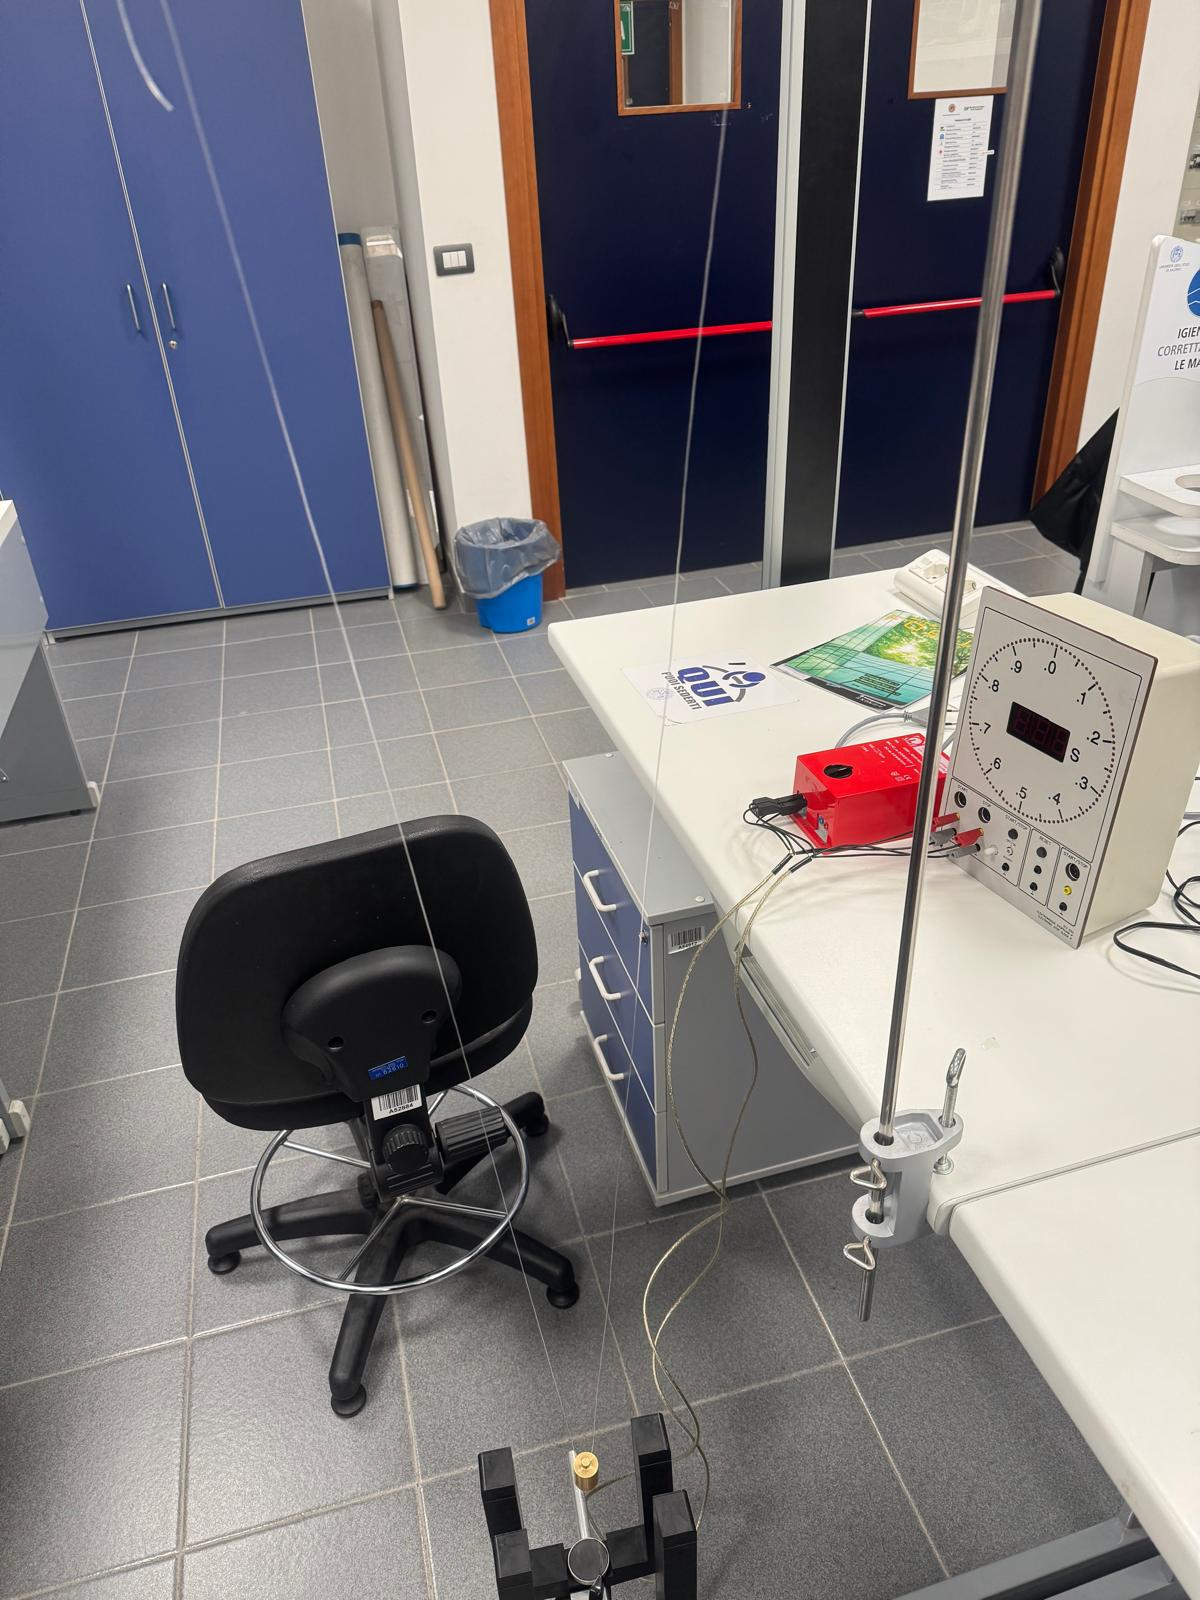
\includegraphics[width=0.55\textwidth]{pendolo.jpg}
  \caption{Pendolo assemblato.}
\end{figure}
\begin{figure}[H]
  \centering
  \subfloat[Cronometro digitale]{%
    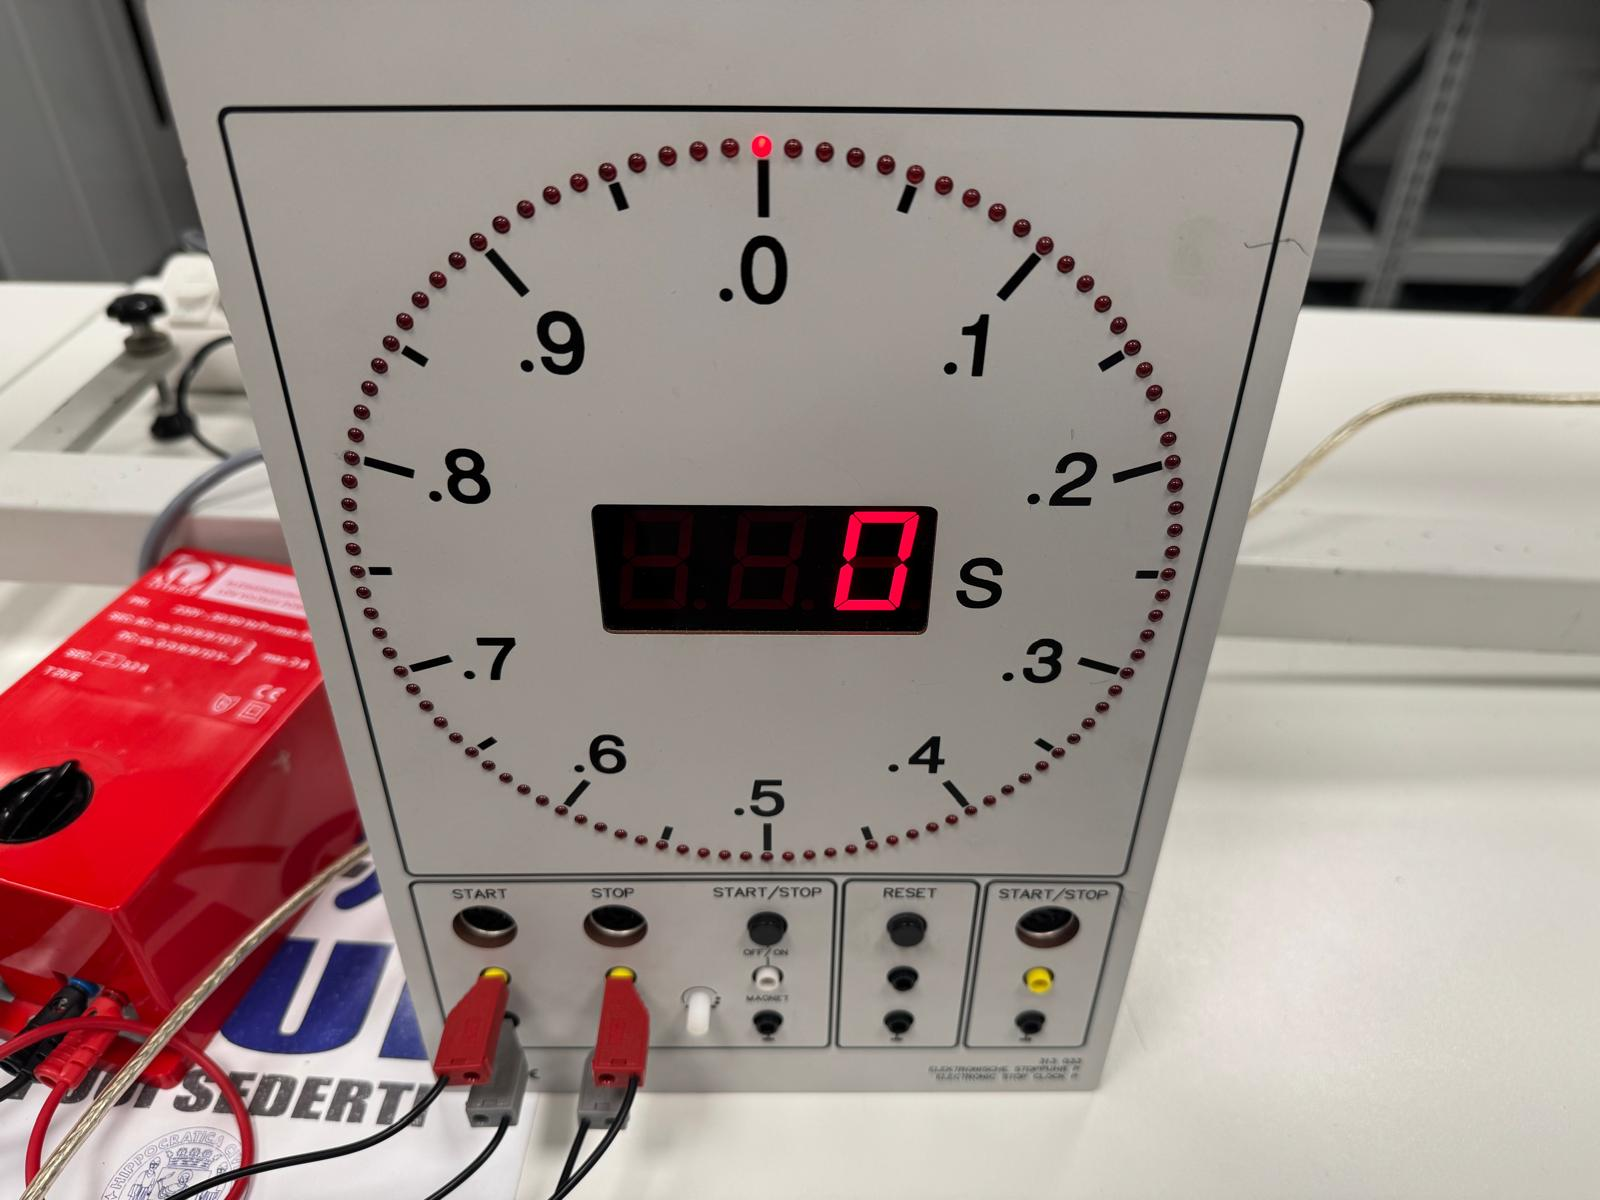
\includegraphics[width=0.45\textwidth]{cronometro.jpg}
  }
  \hspace{0.5cm} % Spazio tra le due immagini
  \subfloat[Metro a nastro]{%
    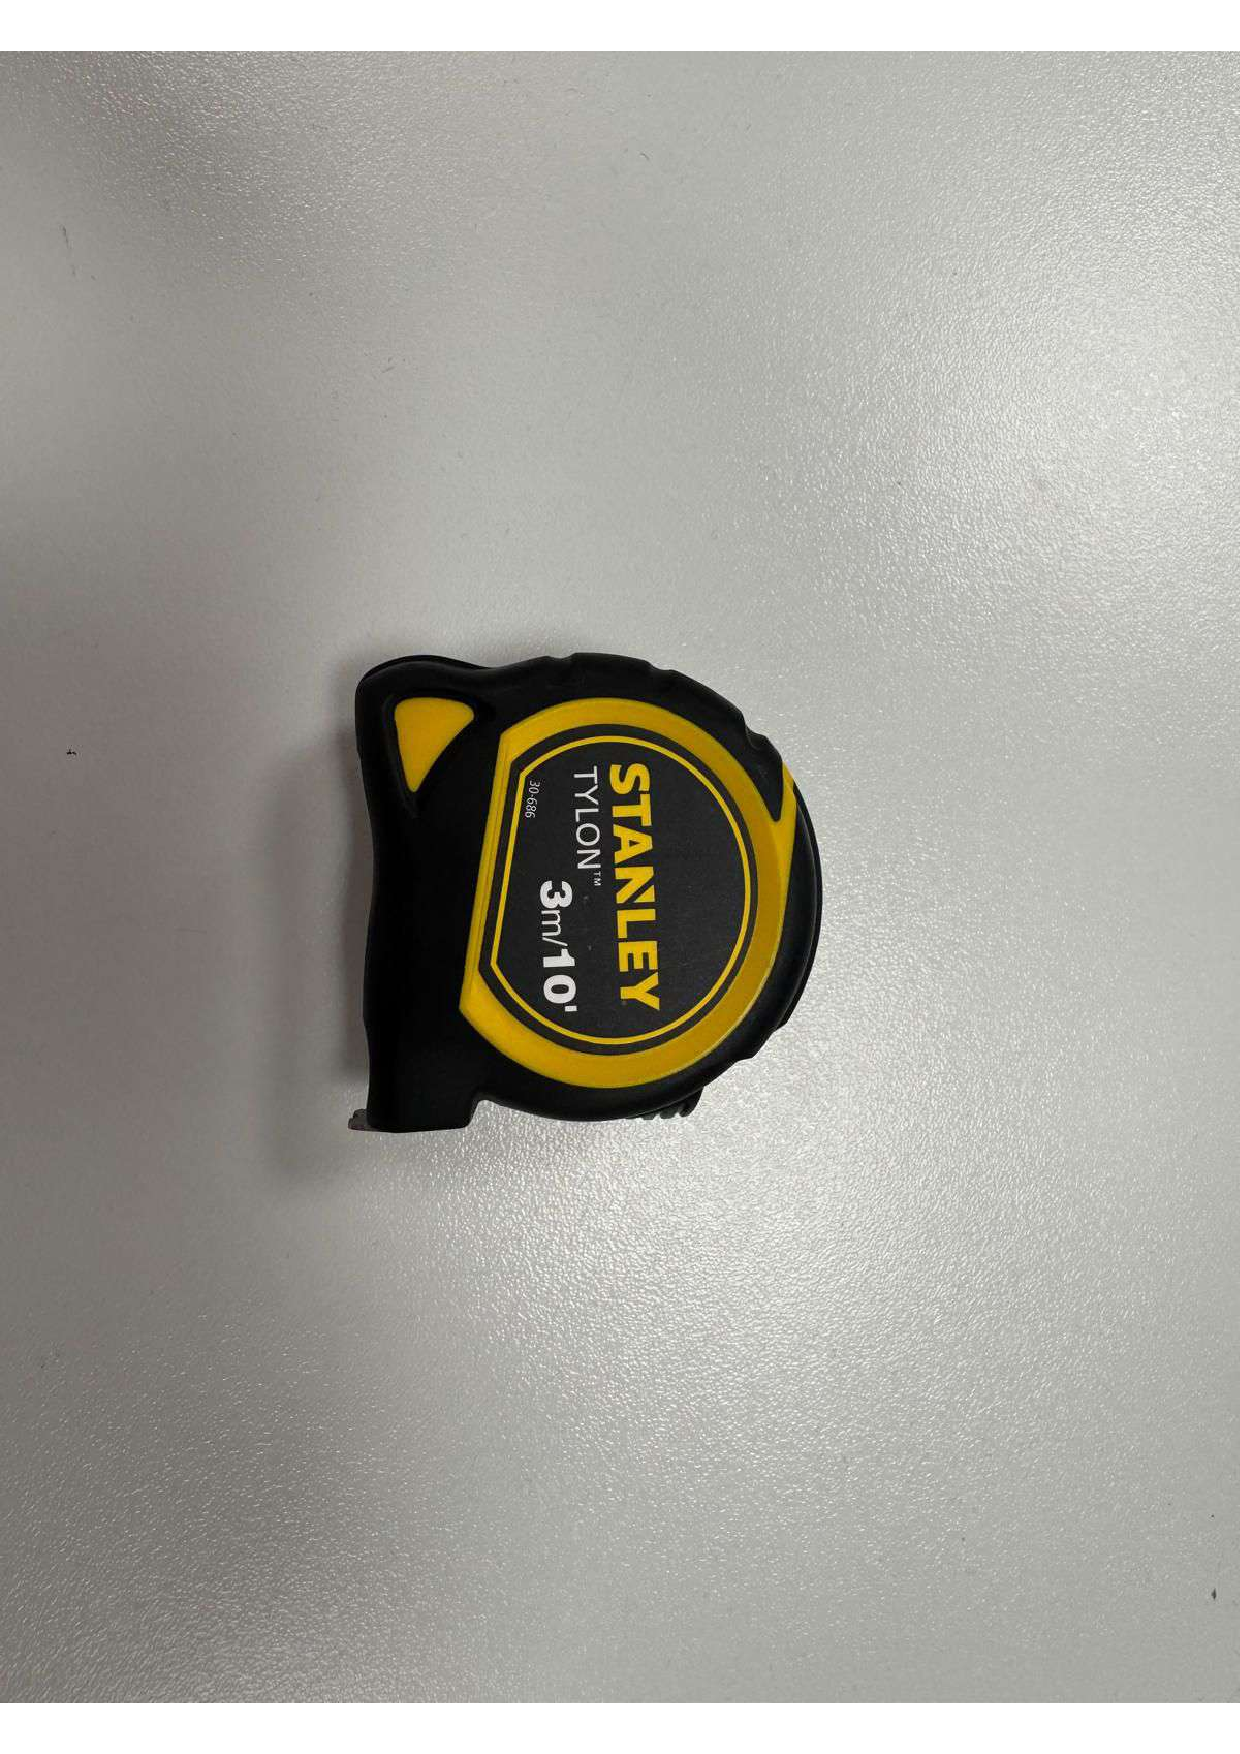
\includegraphics[width=0.45\textwidth]{metro (1).pdf}
  }
  \label{fig:due_immagini}
\end{figure}


\section{Descrizione e analisi dei dati sperimentali}
Abbiamo misurato il semiperiodo di oscillazione per otto ampiezze differenti, facendo attenzione a rimanere al di fuori del range di piccole oscillazioni. L'ampiezza è stata misurata indirettamente, considerando la relazione:
\begin{equation}
    \theta = \arccos\left(\frac{l-h}{l}\right)
\end{equation}
Mentre la sua incertezza, dalla Legge (13) e ponendo $\vec{x_0}=(l,h)$, sarà calcolata con la relazione:
\begin{equation}
    \Delta \theta=\left(\frac{1}{\sqrt{1-\left(\frac{l-h}{l}\right)^2}}\left(\frac{h}{l^2}\right)\right)\Delta l + \left(\frac{1}{\sqrt{1-\left(\frac{l-h}{l}\right)^2}}\left(\frac{1}{l}\right)\right)\Delta h
\end{equation}
\begin{figure}[H]
  \centering
  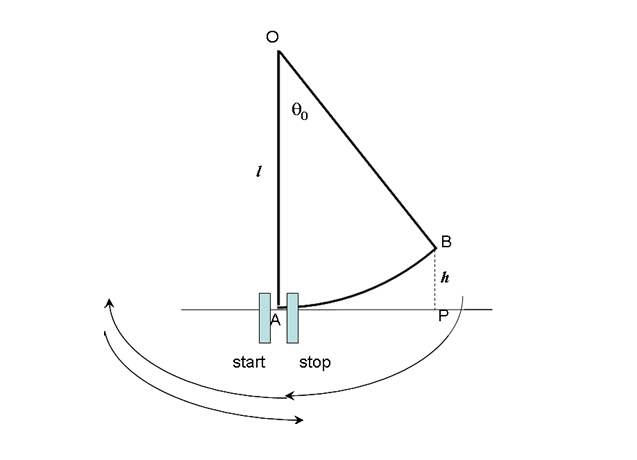
\includegraphics[width=0.55\textwidth]{pendolo1.png}
  \caption{La figura mostra graficamente le grandezze agenti nella Legge (16).}
\end{figure}
Per ognuna delle ampiezze abbiamo ottenuto cinque misurazioni del semiperiodo. Il valore finale è stato ottenuto calcolando la media e valutando l'errore per semidispersione (laddove fosse maggiore dell'errore strumentale). L'altezza $l$ del pendolo è stata fissata a
\begin{equation}
    l=(108\pm 0.05)\ cm
\end{equation}

\subsection{Prima ampiezza}
Con $h_1 = (19.50\pm 0.05)\ cm$ otteniamo, dalla (16) e dalla (17), l'ampiezza:
\begin{equation}
    \theta_1 = (0.61036\pm 0.00096)\ rad
\end{equation}

\begin{table}[H]
\centering
\begin{tabular}{|c|}
\hline
\textbf{T/2 $[s]$} \\
\hline
$1.08\pm 0.01$ \\
$1.08\pm 0.01$ \\
$1.08\pm 0.01$ \\
$1.08\pm 0.01$ \\
$1.08\pm 0.01$ \\
\hline
\end{tabular}
\caption{Semiperiodi misurati per la prima ampiezza.}
\label{tab:}
\end{table}
Il periodo di oscillazione è quindi:
\begin{equation}
    T_1=(2.16\pm 0.02)\ s
\end{equation}

\subsection{Seconda ampiezza}
Con $h_2 = (29.50\pm 0.05)\ cm$ otteniamo, dalla (16) e dalla (17), l'ampiezza:
\begin{equation}
    \theta_2 = (0.75707\pm 0.00086)\ rad
\end{equation}

\begin{table}[H]
\centering
\begin{tabular}{|c|}
\hline
\textbf{T/2 $[s]$} \\
\hline
$1.09\pm 0.01$ \\
$1.09\pm 0.01$ \\
$1.09\pm 0.01$ \\
$1.09\pm 0.01$ \\
$1.09\pm 0.01$ \\
\hline
\end{tabular}
\caption{Semiperiodi misurati per la seconda ampiezza.}
\label{tab:}
\end{table}
Il periodo di oscillazione è quindi:
\begin{equation}
    T_2=(2.18\pm 0.02)\ s
\end{equation}

\subsection{Terza ampiezza}
Con $h_3= (39.50\pm 0.05)\ cm$ otteniamo, dalla (16) e dalla (17), l'ampiezza:
\begin{equation}
    \theta_3 = (0.88375\pm 0.00082)\ rad
\end{equation}

\begin{table}[H]
\centering
\begin{tabular}{|c|}
\hline
\textbf{T/2 $[s]$} \\
\hline
$1.10\pm 0.01$ \\
$1.10\pm 0.01$ \\
$1.10\pm 0.01$ \\
$1.10\pm 0.01$ \\
$1.10\pm 0.01$ \\
\hline
\end{tabular}
\caption{Semiperiodi misurati per la terza ampiezza.}
\label{tab:}
\end{table}
Il periodo di oscillazione è quindi:
\begin{equation}
    T_3=(2.20\pm 0.02)\ s
\end{equation}

\subsection{Quarta ampiezza}
Con $h_4=(44.50\pm 0.05)\ cm$ otteniamo, dalla (16) e dalla (17), l'ampiezza:
\begin{equation}
    \theta_4= (0.94226\pm 0.00081)\ rad
\end{equation}

\begin{table}[H]
\centering
\begin{tabular}{|c|}
\hline
\textbf{T/2 $[s]$} \\
\hline
$1.11\pm 0.01$ \\
$1.11\pm 0.01$ \\
$1.11\pm 0.01$ \\
$1.11\pm 0.01$ \\
$1.11\pm 0.01$ \\
\hline
\end{tabular}
\caption{Semiperiodi misurati per la quarta ampiezza.}
\label{tab:}
\end{table}
Il periodo di oscillazione è quindi:
\begin{equation}
    T_4=(2.22\pm 0.02)\ s
\end{equation}

\subsection{Quinta ampiezza}
Con $h_5=(49.50\pm 0.05)\ cm$ otteniamo, dalla (16) e dalla (17), l'ampiezza:
\begin{equation}
    \theta_5 = (0.99838\pm 0.00081)\ rad
\end{equation}

\begin{table}[H]
\centering
\begin{tabular}{|c|}
\hline
\textbf{T/2 $[s]$} \\
\hline
$1.12\pm 0.01$ \\
$1.12\pm 0.01$ \\
$1.12\pm 0.01$ \\
$1.12\pm 0.01$ \\
$1.12\pm 0.01$ \\
\hline
\end{tabular}
\caption{Semiperiodi misurati per la quinta ampiezza.}
\label{tab:}
\end{table}
Il periodo di oscillazione è quindi:
\begin{equation}
    T_5=(2.24\pm 0.02)\ s
\end{equation}

\subsection{Sesta ampiezza}
Con $h_6=(62.00\pm 0.05)\ cm$ otteniamo, dalla (16) e dalla (17), l'ampiezza:
\begin{equation}
    \theta_6=(1.13081\pm 0.00081)\ rad
\end{equation}

\begin{table}[H]
\centering
\begin{tabular}{|c|}
\hline
\textbf{T/2 $[s]$} \\
\hline
$1.14\pm 0.01$ \\
$1.14\pm 0.01$ \\
$1.14\pm 0.01$ \\
$1.14\pm 0.01$ \\
$1.14\pm 0.01$ \\
\hline
\end{tabular}
\caption{Semiperiodi misurati per la sesta ampiezza.}
\label{tab:}
\end{table}
Il periodo di oscillazione è quindi:
\begin{equation}
    T_6=(2.28\pm 0.02)\ s
\end{equation}

\subsection{Settima ampiezza}
Con $h_7=(79.50\pm 0.05)\ cm$ otteniamo, dalla (16) e dalla (17), l'ampiezza:
\begin{equation}
    \theta_7=(1.30375\pm 0.00084)\ rad
\end{equation}

\begin{table}[H]
\centering
\begin{tabular}{|c|}
\hline
\textbf{T/2 $[s]$} \\
\hline
$1.17\pm 0.01$ \\
$1.17\pm 0.01$ \\
$1.17\pm 0.01$ \\
$1.17\pm 0.01$ \\
$1.17\pm 0.01$ \\
\hline
\end{tabular}
\caption{Semiperiodi misurati per la settima ampiezza.}
\label{tab:}
\end{table}
Il periodo di oscillazione è quindi:
\begin{equation}
    T_7=(2.34\pm 0.02)\ s
\end{equation}

\subsection{Ottava ampiezza}
Con $h_8= (89.50\pm 0.05)\ cm$ otteniamo, dalla (16) e dalla (17), l'ampiezza:
\begin{equation}
    \theta_8 = (1.39865\pm 0.00086)\ rad
\end{equation}

\begin{table}[H]
\centering
\begin{tabular}{|c|}
\hline
\textbf{T/2 $[s]$} \\
\hline
$1.19\pm 0.01$ \\
$1.19\pm 0.01$ \\
$1.19\pm 0.01$ \\
$1.19\pm 0.01$ \\
$1.19\pm 0.01$ \\
\hline
\end{tabular}
\caption{Semiperiodi misurati per l'ottava ampiezza.}
\label{tab:}
\end{table}
Il periodo di oscillazione è quindi:
\begin{equation}
    T_8=(2.18\pm 0.02)\ s
\end{equation}

\subsection{Elaborazione}
Per ottenere il valore di $g$ abbiamo posto, in un grafico, il periodo di oscillazione in funzione del quadrato dell'ampiezza (Vedi Legge (2)).
\begin{figure}[H]
  \centering
  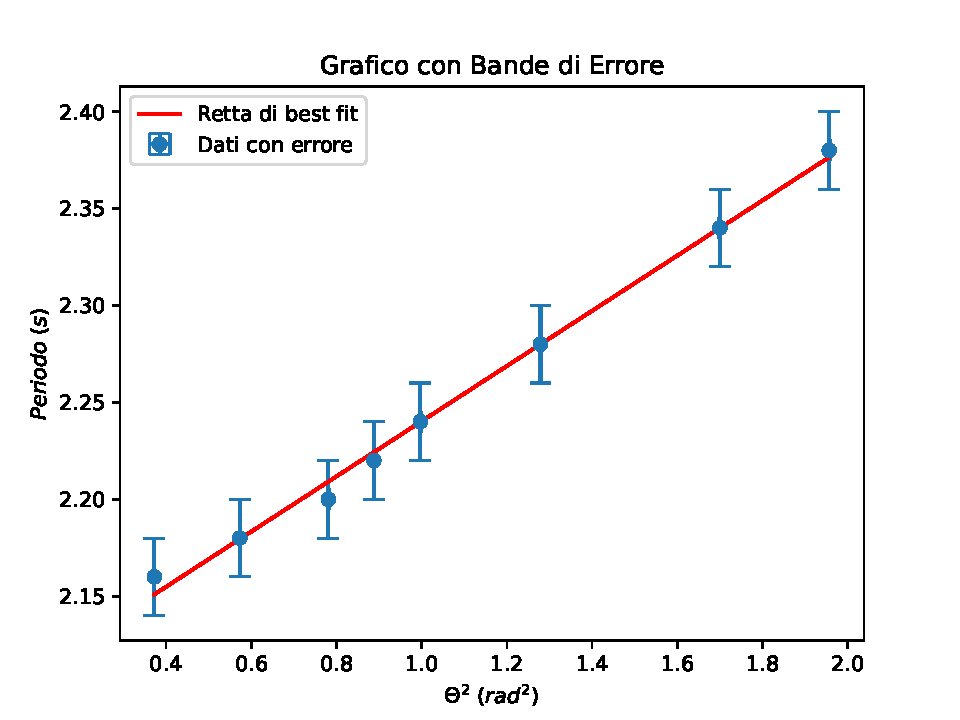
\includegraphics[width=0.95\textwidth]{grafico1.pdf}
  \caption{Il grafico mostra il periodo di oscillazione in funzione del quadrato dell'ampiezza. \\
  Coefficiente angolare: $(0.142\pm 0.012)\ s\\$
  Intercetta: $(2.098\pm 0.014)\ s$\\
  Questi parametri sono stati ottenuti utilizzando il metodo dei minimi quadrati (vedi Paragrafo 2.1).}
\end{figure}

\section{Conclusioni}
In conclusione ci è possibile stabilire una stima di $g$ partendo dalla Legge (2). Riscrivendola, eseguendo il prodotto, otteniamo:
\begin{equation}
    T=\left(2\pi\sqrt{\frac{l}{g}}\right)+\left(\frac{2\pi}{16}\sqrt{\frac{l}{g}}\theta_{max}^2\right)
\end{equation}
che è rappresentata dalla retta di regressione in Figura (3), in cui:
\begin{itemize}
    \item $Intercetta = \left(2\pi\sqrt{\frac{l}{g}}\right)$
    \item $Coeff. angolare= \left(\frac{2\pi}{16}\sqrt{\frac{l}{g}}\right)$
\end{itemize}

Dall'intercetta ($a$) possiamo ricavare facilmente la g dall'espressione
\begin{equation}
    g_0=\frac{4\pi^2 l}{a^2}
\end{equation}
e la sua incertezza (vedi Legge (13))
\begin{equation}
    \Delta g = \left(\frac{\Delta l}{l} + 2\frac{\Delta a}{a}\right)g_0
\end{equation}
Da cui otteniamo
\begin{equation}
    g = (9.69\pm 0.14) \frac{m}{s^2}
\end{equation}
che rappresenta un'ottima stima dell'accelerazione gravitazionale (valore di riferimento: $g=9.81\frac{m}{s^2}$).

\end{document}